\documentclass[twoside]{article}
\usepackage{amsmath,amssymb,amsthm,graphicx}
\usepackage{epsfig}
\usepackage[authoryear]{natbib}

\newcommand{\reals}{\mathbf{R}}
\newcommand{\integers}{\mathbf{Z}}
\newcommand{\naturals}{\mathbf{N}}
\newcommand{\rationals}{\mathbf{Q}}

% Caligraphic alphabet
\newcommand{\calr}{\mathcal{R}} % only because \cr already taken
\newcommand{\ca}{\mathcal{A}} \newcommand{\cb}{\mathcal{B}} \newcommand{\cc}{\mathcal{C}} \newcommand{\cd}{\mathcal{D}} \newcommand{\ce}{\mathcal{E}} \newcommand{\cf}{\mathcal{F}} \newcommand{\cg}{\mathcal{G}} \newcommand{\ch}{\mathcal{H}} \newcommand{\ci}{\mathcal{I}} \newcommand{\cj}{\mathcal{J}} \newcommand{\ck}{\mathcal{K}} \newcommand{\cl}{\mathcal{L}} \newcommand{\cm}{\mathcal{M}} \newcommand{\cn}{\mathcal{N}} \newcommand{\co}{\mathcal{O}} \newcommand{\cp}{\mathcal{P}} \newcommand{\cq}{\mathcal{Q}} \newcommand{\cs}{\mathcal{S}} \newcommand{\ct}{\mathcal{T}} \newcommand{\cu}{\mathcal{U}} \newcommand{\cv}{\mathcal{V}} \newcommand{\cw}{\mathcal{W}} \newcommand{\cx}{\mathcal{X}} \newcommand{\cy}{\mathcal{Y}} \newcommand{\cz}{\mathcal{Z}}

\newcommand{\ind}[1]{1_{#1}} % Indicator function
\newcommand{\pr}{\mathbb{P}} % Generic probability
\newcommand{\ex}{\mathbb{E}} % Generic expectation
\newcommand{\var}{\textrm{Var}}
\newcommand{\cov}{\textrm{Cov}}
\newcommand{\sign}{\textrm{sign}}
\newcommand{\kl}{\textrm{KL}} 

\newcommand{\law}{\mathcal{L}}  % \law{X}, the measure associated with r.v. X
\newcommand{\normal}{N} % for normal distribution (can probably skip this)
\newcommand{\eps}{\varepsilon}

% Convergence
\newcommand{\convd}{\stackrel{d}{\longrightarrow}} % convergence in distribution/law/measure
\newcommand{\convp}{\stackrel{p}{\longrightarrow}} % convergence in probability
\newcommand{\convas}{\stackrel{\textrm{a.s.}}{\longrightarrow}} % convergence almost surely

\newcommand{\eqd}{\stackrel{d}{=}} % equal in distribution/law/measure
\newcommand{\argmax}{\textrm{argmax}}
\newcommand{\argmin}{\textrm{argmin}}
\newcommand{\conv}{\textrm{conv}} % for denoting the convex hull

% Theorem-like declarations
\theoremstyle{plain}
\newtheorem{theorem}{Theorem}
\newtheorem{corollary}[theorem]{Corollary}
\newtheorem{lemma}[theorem]{Lemma}

\theoremstyle{definition}
\newtheorem{definition}[theorem]{Definition}
\newtheorem{example}[theorem]{Example}

\theoremstyle{remark}
\newtheorem{remark}[theorem]{Remark}



\setlength{\oddsidemargin}{0.25 in}
\setlength{\evensidemargin}{-0.25 in}
\setlength{\topmargin}{-0.6 in}
\setlength{\textwidth}{6.5 in}
\setlength{\textheight}{8.5 in}
\setlength{\headsep}{0.75 in}
\setlength{\parindent}{0 in}
\setlength{\parskip}{0.1 in}

\newcommand{\lecture}[4]{
   \pagestyle{myheadings}
   \thispagestyle{plain}
   \newpage
   \setcounter{page}{1}
   \noindent
   \begin{center}
   \framebox{
      \vbox{\vspace{2mm}
    \hbox to 6.28in { {\bf 6.882:~Bayesian Modeling and Inference \hfill Lecture Date: #4} }
       \vspace{6mm}
       \hbox to 6.28in { {\Large \hfill #1  \hfill}  }
       \vspace{6mm}
       \hbox to 6.28in { {\it Lecturer: #2 \hfill Scribe: #3} }
      \vspace{2mm}}
   }
   \end{center}
   \markboth{#1}{#1}
   \vspace*{4mm}
}

% Local Macros Put your favorite macros here that don't appear in
% stat-macros.tex.  We can eventually incorporate them into
% stat-macros.tex if they're of general use.

\begin{document}

\lecture{The Indian Buffet Process: An Introduction and Review}{Alternative Scribe}{Genevieve Flaspohler}{April 18, 2017}


\section{Background}
\label{sec:back}
This background section was adapted from the introduction in \citet{Blei2010}.

Most methods within the field of machine learning can be divided between supervised and unsupervised problems. In supervised problems, we are provided with data and an associated label. The crux of these algorithms is to find a suitably robust and accurate function that maps from our data space $\cal X$ to our label space $\cal Y$, $f: \cal X \to \cal Y$. Unsupervised learning tackles a fundamentally different, and perhaps more challenging, problem. Given only the data, unsupervised learning seeks to infer useful structure or patterns within this data. Classical unsupervised learning problems include clustering and dimension reduction. 

In supervised learning problems, the data labels provide the problem with enough structure to learn a meaningful function $f$. In unsupervised learning, this structure is not inherent in the data, and the problem designer must provide structure in the form of probabilistic generative models. These generative models define what "structure" or "pattern" means in the context of the data. Generative models are often specified in the form of a probabilistic graphical model, allowing inference and belief updates to take place within a fully Bayesian framework.

In this class, we have learned about several unsupervised learning models and their generative processes. For example, the Latent Dirichlet Allocation (LDA) specifies a generative process where data are modeled as a collection of documents, each of which is generated from a mixture of global topics (Fig. \ref{fig:graph}). Bayesian inference in this model is then tractable because of the conditional contumacy relationships embedded in the LDA graphical model.

\begin{figure}[h]
  \centering
    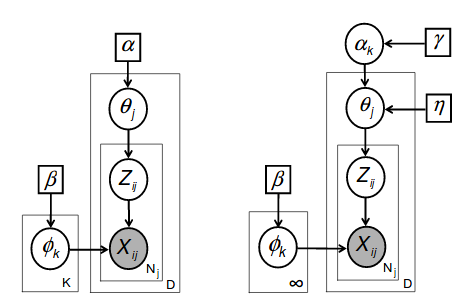
\includegraphics[scale=0.45]{hdp_lda}
    \caption{Caption me.\citet{Newman}}
  \label{fig:hdp_lda}
\end{figure}

LDA is an example of a parametric unsupervised learning model; the number of global topics present in the data $K$ is pre-specified and cannot grow to accommodate additional data. Since the majority of the structure in unsupervised learning problems is imposed by the generative model, a generative model with strong, parametric assumptions will tend to inform the discovered structure more than the data itself. Additionally, many data have a fundamentally growing number of parameters: the more documents you analyze, the more topics you are likely to discover; the more animals you find on earth, the more species you will discover. These data could not be accommodated by a parametric model.

Bayesian nonparametric (BNP) inference seeks to overcome these limitations.  BNP models replace parametric priors and posteriors with stochastic processes. Stochastic processes are infinite, indexed collections of random variables. By allowing the number of parameters to be unbounded and grow with the data, BNP models provide the weakest assumptions possible, allowing the ``data to speak", while still providing enough structure to learning meaningful patterns in the data. In this class, we have seen serveral BNP models. For example, the HDP topic model, a nonparametric extension of LDA, employs a nested Dirichlet process to allow the number of global topics within the corpus to be determined by the data (Fig. \ref{fig:graph}). 

\section{Motivation}
The problem we will explore in these notes is that of data clustering and cluster property inference. For example, given data generated from a mixture of three Gaussian distributions, we would wish to infer the clutter membership of each data point and the mean and variance of each cluster. A Dirichlet process (DP) and its marginal, the Chinese Restaurant Process (CRP) provide an elegant nonparmetric solution to this cluster problem (Fig .\ref{fig:cluster}). 

\begin{figure}[h]
  \centering
    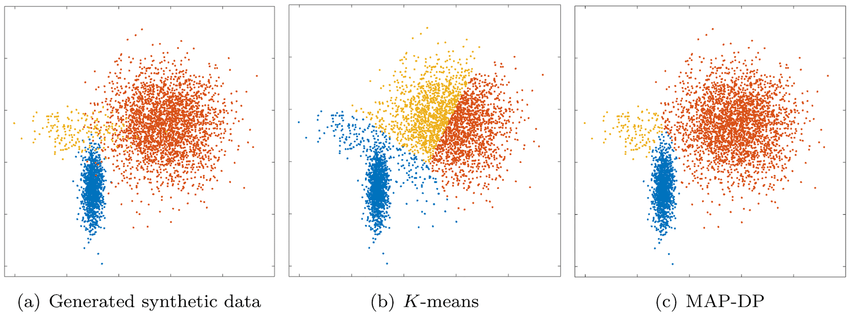
\includegraphics[scale=0.35]{cluster}
    \caption{Caption me.\citet{Raykov2016}}
  \label{fig:graph}
\end{figure}

As we have seen in Section \ref{sec:back}, the structure imposed on an unsupervised learning problem, via a generative process, plays a critical role in the underlying patterns discovered in the data. Given identical data, different generative processes will infer different latent structures in the data. For our clustering problem, the DP structure models each data point as being generated from only one cluster and its observable properties are determined solely by this cluster identify. For some data, this assumption is too limiting.  The Beta process, and its marginal the Indian Buffet Process (IBP), introduces a more flexible generative model. Under the IBP, each data point can belong to many different classes (i.e. features) and the point's final observable properties are determined by a combination of the influences of all of its features.  

The difference between the structure imposed by the CRP and the IBP is highlighted in Figure \ref{fig:ibp_crp}. In the CRP, a data point (customer) is identified with a single cluster (table) and the data point's properties are entirely determined by that cluster. In the IBP, each data point (customer) can be associated with a potentially infinite number of dishes (features), which influence the data point's expression. We will explore the formulation of the IBP generative process and its implications on the discovered latent structure in data in the rest of the notes.

\begin{figure}[h]
  \centering
    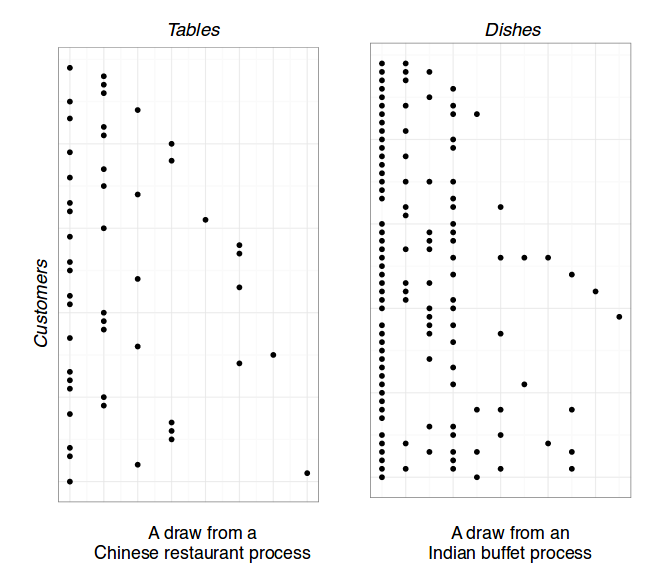
\includegraphics[scale=0.40]{crp_vs_ibp}
    \caption{Caption me.\citet{Gershman2011}}
  \label{fig:ibp_crp}
\end{figure}

\section{Indian Buffet Process Model}
In \citet{Griffiths2011}, the authors define the Indian Buffet Process (IBP) as: "a stochastic process defining a probability distribution over equivalence classes of sparse binay matrices with a finite number of rows and an unbounded number of columns." I will expand upon this definition and the problem set up in the following section; however, the matrix in Figure \ref{fig:ibp_crp} is a good one to keep in mind.

\subsection{Latent Class Models}
In the classical clustering problem, we have $N$ objects, with the $i$th object having $D$ observable properties represented by a row vector $\mathbf{x_i}$. Our $N \times D$ data matrix $\mathbf{X} = [\mathbf{x_1^T x_2^T \dots x_N^T}]$ indicates the properties of all $N$ objects. In a mixture model, where each data point can only belong to one class, we would also define a class vector $\mathbf{c} = [c_1 c_2 \dots c_N]^T$ to indicate the class membership of each data point. A mixture model would then be specified by a prior over class assignments $P(\mathbf{c})$ and the likelihood of our data given the class assignments $P(\mathbf{X | c})$. In the IBP model, we will modify both the prior and the likelihood function to allow each data point to be associated with an unbounded number of classes.

\subsection{Latent Feature Models}
In a latent feature model, we again have $N$ objects, with the $i$th object having $D$ observable properties represented by a row vector $\mathbf{x_i}$. However, we now assume that these properties are generated from a distribution determined by a latent feature vector $\mathbf{f_i}$ associated with each data point. Instead of a class vector, we now have a feature matrix $\mathbf{F} = [\mathbf{f_1^T f_2^T \dots f_N^T}]$. Our model is now specified with the corresponding prior over features $P(\mathbf{F})$ and the likelihood of our observed properites given the features, $P(\mathbf{X | C})$.

In this work, the prior over features $P(\mathbf{F})$ is broken into two component matrices: a binary matrix $\mathbf{Z}$ that indicates if a feature is possessed by each data point, and a matrix $\mathbf{V}$ which indicates the value of the feature for each data point. This decomposition is visualized in Figure \ref{fig:decomp}. The paper focuses on defining a prior over $\mathbf{Z}$, since knowing $\mathbf{Z}$ is sufficient to determine the dimension of $\mathbf{V}$ and therefore $\mathbf{F}$.

\begin{figure}[h]
  \centering
    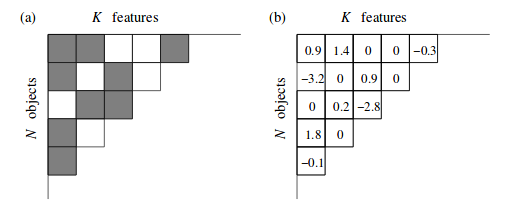
\includegraphics[scale=0.70]{fzv}
  \caption{Caption me.}
  \label{fig:decomp}
\end{figure}

\subsection{Defining a prior over infinite binary matrices}
In our previous nonparametric clustering problem, we have seen a prior over an unbounded number of clusters defined in a variety of ways (e.g. as the limit of a finite model or via a simple stochastic process - the CRP). We can also definite our desired prior $P(\mathbf{Z})$ in these two ways, as we will see in the following sections.

\subsubsection{Defining via stochastic process (IBP)}
Just as in the CRP, we can definite our prior over infinite binary matrices using a simple stochastic process. In the Indian Buffet Process (IBP), $N$ customers enter the customer one after another. Each customer is presented with a buffet of infinitely many dishes in a line. The first customer starts with the leftmost dish and samples the next $\text{Poisson}(\alpha)$ dishes. The next customer samples each of the dishes sampled by the first customer with probability $\frac{m_k}{i}$, where $m_k$ is the number of customers who have sampled dish $k$ so far and $i$ is the total number of previous customers. She then chooses an additional $\text{Poisson}(\frac{\alpha}{i})$ new dishes to the right of the dishes sampled so far. This process repeats for all $N$ customers.

We can use an $N \times K$ binary matrix to represent the customers' dish choices (this matrix corresponds to the $\mathbf{Z}$ matrix necessary for the latent feature model). This matrix will have a finite number of rows (customers) and a potentially infinite number of columns (dishes).  An example of the matrix produced using $\alpha = 10$ is shown in Figure \ref{fig:ex}. In this matrix, the first customer tries 17 dishes. The second customer sampled 7 of those dishes and three new dishes. The process was repeated for a total of 20 customers.

\begin{figure}[h]
  \centering
  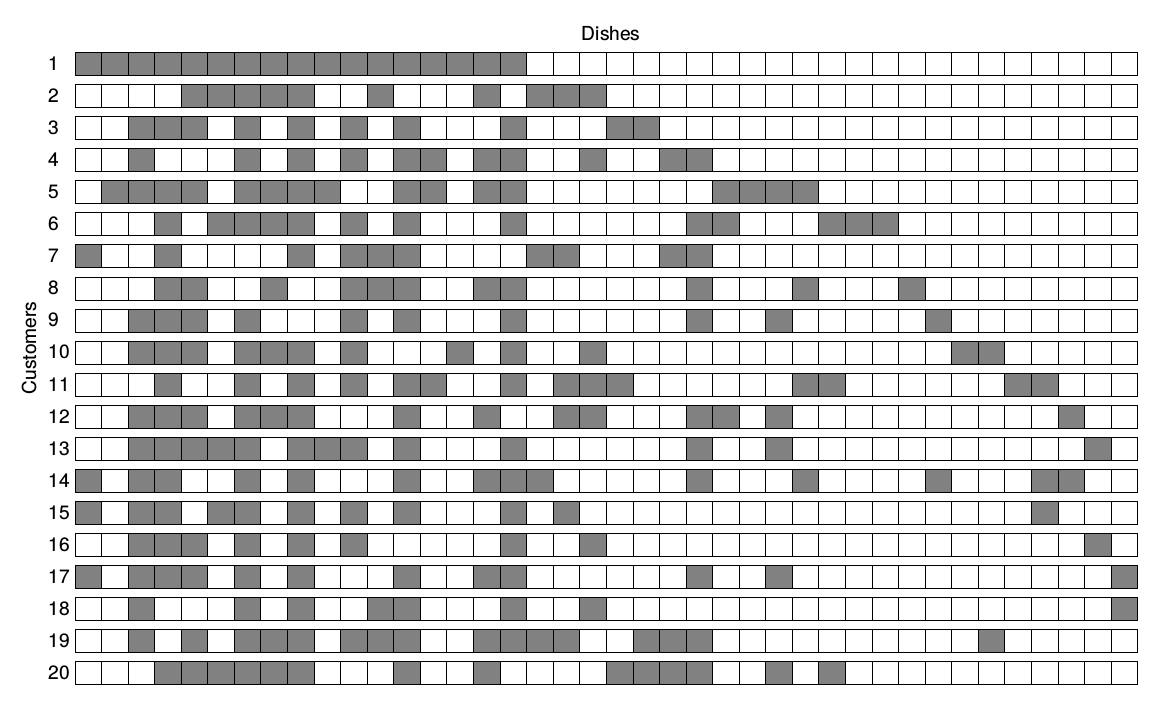
\includegraphics[scale=0.35]{ex}
  \caption{Caption me.}
  \label{fig:ex}
\end{figure}

We can calculate the probability of a particular matrix being produced by the IBP as

\begin{equation}
    P(\mathbf{Z}) = \frac{\alpha^{K+}}{\prod_{i = 1}^{N}K_1^{(i)}!} \exp\{-\alpha H_N\} \prod_{k = 1}^{K+} \frac{(N-m_k)!(m_k-1)!}{N!}
    \label{eq:ibp}
\end{equation}

where $K+$ is the largest number dish that some customer previously sampled, $K_1^{(i})$ indicates the number of new dishes samples by the $i$th customer and $H_N$ is the $N$th harmonic number.

\subsubsection{Defining as limit of finite model}
Alternatively, we can define a prior over infinite binary matrices as the limit of a prior over finite binary matrices. In this section, we assume a model with a finite number of features $K$, and then take the limit as $K \to \infty$. We have $N$ objects, each with $K$ features. The indicator variable $z_{ik}$ indicates whether object $i$ possess feature $k$. Each object independently possess feature $k$ with probability $\pi_k$. Under this model, the probability of a matrix $\mathbf{Z}$ given $\pi = \{\pi_1, \pi_2, \dots \pi_K\}$ is
\begin{equation}
    P(\mathbf{Z} | \pi) = \prod_{k = 1}^K \prod_{i = 1}^N P(z_{ik} | \pi_k) = \prod_{k = 1}^K \pi_k^{m_k} (1 - \pi_k)^{N-m_k}
\end{equation}
where $m_k = \sum_{i=1}^N z_{ik}$ is the number of objects processing feature $k$.

In order to do Bayesian inference, given this likelihood, we need to define a prior on $\pi$. In the paper, they let each $\pi_k$ be drawn from a Beta distribution with parameters $r, s$. Letting $r = \frac{\alpha}{K}$ and $s = 1$, we have the following probability model:
\begin{equation}
\begin{split}
    \pi_k | \alpha & \sim \text{Beta}(\frac{\alpha}{K}, 1) \\
    z_{ik} | \pi_k & \sim \text{Bernoulli}(\pi_k)
\end{split}
\end{equation}

Given this model, we can integrate out $\pi$ and find the marginal probability for $\mathbf{Z}$:
\begin{equation}
\begin{split}
    P(\mathbf{Z}) & = \prod_{k = 1}^K \int \prod_{i = 1}^N P(z_{ik} | \pi_k) P(\pi_k) d\pi_k \\
    &  = \prod_{k = 1}^K \frac{\frac{\alpha}{K} \Gamma(m_k + \frac{\alpha}{K}) \Gamma(N - m_k + 1)}{\Gamma(N + 1 + \frac{\alpha}{K})} \\
\end{split}
\label{eq:pz}
\end{equation}

We will now explore what happens to these equations as we take the limit $K \to \infty$.

\subsubsection*{Note: Equivalence classes}
When we talk about the probability of a specific feature matrix $\mathbf{Z}$, what we really want to define is the probability over a specific, exchangeable equivalence class of feature matrices. In the CRP model, we said that the order in which customers were assigned to tables did not matter. Every ordering that led to the same partition of the customers into tables was equivalent. Theses orderings formed an equivalence class, and we defined probabilities of partitions of customers, not specific orderings of assigning customers to tables. 

\begin{figure}[h]
  \centering
    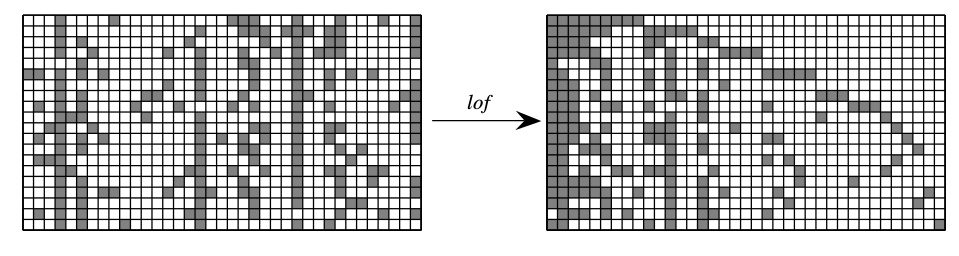
\includegraphics[scale=0.35]{lof}
  \caption{Caption me.}
  \label{fig:lof}
\end{figure}

We want to define a similar equivalence classes for binary matrices, so that we can talk about the probability of equivalence classes instead of individual matrices. The authors introduced an equivalence classes based on a binary matrix's \textit{left-ordered form}. After applying the many-to-one \textit{lof()} function, all matrices in the same equivalence class will collapse to an identical matrix. The \textit{lof()} function is shown in Figure \ref{fig:lof}. 

Using Eq. \ref{eq:pz}, we can define the probability of an equivalence class of matrices $[\mathbf{Z}]$ as

\begin{equation}
\begin{split}
    P([\mathbf{Z}]) & = \sum_{\mathbf{Z} \in [\mathbf{Z}]} P(\mathbf{Z}) \\
    & = \frac{K!}{\prod_{h = 0}^{2^{N-1}}K_h!}\prod_{k=1}^K \frac{\frac{\alpha}{K} \Gamma(m_k + \frac{\alpha}{K}) \Gamma(N - m_k + 1)}{\Gamma(N + 1 + \frac{\alpha}{K})}
\end{split}
    \label{eq:pe}
\end{equation}

Taking the limit of Eq. \ref{eq:pe} as $K \to \infty$, we are left with the following expression for $P([\mathbf{Z}])$:

\begin{equation}
    P([\mathbf{Z}]) = \frac{\alpha^{K+}}{\prod_{h = 1}^{2^{N-1}}K_h!} \exp\{-\alpha H_N\} \prod_{k = 1}^{K+} \frac{(N-m_k)!(m_k-1)!}{N!}
    \label{eq:limit}
\end{equation}
where $K+$ is the number of columns for which there is at least one data point with that feature and $H_N$ is the $N$th harmonic number. Further details of these derivations can be found in \citet{Griffiths2011}.

Note that this form is slightly different than the probability introduced by the IBP in Eq. \ref{eq:ibp}. However, the probability in Eq. \ref{eq:ibp} was defined for a specific matrix, not over \textit{lof()} equivalence classes.  The matrices produced by the IBP are not in left-order form, but are also not random, because customers choose dishes starting at the left side of the buffet. Therefore, there are $\frac{\prod_{i=1}^N K_1^{(i)}!}{\prod_{h=1}^{2^{N-1}} K_h!}$ matrices generated by the IBP that map to the same left-ordered from. When this number is used to find the corresponding $P([\mathbf{Z}])$ for Eq. \ref{eq:ibp} from the IBP, the result will be identical to Eq. \ref{eq:limit}. 

\subsubsection{Properties of IBP}
We have now defined two processes to construct a prior over our infinite binary feature matrix $\mathbf{Z}$. Defined in this way, $\mathbf{Z}$ has some interesting properties:
\begin{itemize}
    \item The effective dimension of the model, $K+$ grows as $\text{Poisson}(\alpha H_N)$.
    \item The number of features possessed by each object follows a Poisson($\alpha$) distribution.
    \item The matrix $\mathbf{Z}$ will remain sparse as $K \to \infty$. The expected number of entries in $\mathbf{Z}$ is $N\alpha$.
\end{itemize}

\subsection{Inference in the IBP Model}
\label{sec:gibbs}
From the above sections, we know how to construct a prior over infinite, sparse, binary matrices that represent the presence/absence of an unbounded number of features in our $N$ data points. The next important question to ask is whether inference is tractable under such an infinite model. 

Given observed data $\mathbf{X}$, the authors introduce a Gibbs sampler for inferring the posterior $P(\mathbf{Z | X})$ from our derived prior $P(\mathbf{Z})$ and a likelihood model. To sample from the desired posterior, we need to compute the conditional distributions $P(z_{ik} = 1| \mathbf{Z}_{-(ik)})$. Because the IBP is exchangeable, we choose the current customer $i$ to be the last customer to visit the buffet. This gives us
\begin{equation}
    P(z_{ik} = 1 | \mathbf{z}_{-i, k}) = \frac{m_{-i, k}}{N}
    \label{eq:dish}
\end{equation}
for any $k$ such that $m_{-i, k} > 0$. This leads to the following inference procedure:
\begin{enumerate}
  \item Initialize with an arbitrary binary matrix 
  \item For each row (customer) in the matrix, $i$ 
    \begin{enumerate}
        \item For each column (dish) in the matrix, $k$
            \begin{enumerate}
                \item If $m_{-i, k} > 0$,  set $z_{ik = 1}$ with probability given by Eq. \ref{eq:dish} and incorporate the likelihood $P(\mathbf{X|Z})$.
                \item Otherwise, delete column $k$
            \end{enumerate}
        \item At the end of each row, add $M$ new columns of 1's in that row, where $M \sim \text{Poisson}(\frac{\alpha}{N}) P(\mathbf{X|Z})$.
    \end{enumerate}
\end{enumerate}

After a sufficient burn-in period, the matrix generated will be sampled from the posterior $P(\mathbf{Z|X})$.

\subsection{Examples: Linear-Gaussian Latent Feature Model}
The authors apply the IBP prior to a linear-Gaussian latent feature model with binary features. They start with describe a finite model, and take the model's infinite limit. In the finite model, each data point $\mathbf{x_i}$ is represented by a $D$-dimensional observeable properties vector. Given a $K$-dimensional binary vector $\mathbf{z_i}$, these properties are generated from a Gaussian with mean $\mathbf{z_iA}$ and diagonal covarience matrix $\Sigma_x = \sigma_x^2\mathbf{I}$, where $\mathbf{A}$ is a $K \times D$ matrix of weights.

Our likelihood function $P(\mathbf{X|Z})$ is therefore Gaussian:
\begin{equation}
    P(\mathbf{X|Z, A}, \sigma_x) = \frac{1}{(w\pi\sigma_x^2)^{(ND/2)}}\text{exp}\{\frac{1}{2\sigma_x^2} \text{tr}((\mathbf{X-ZA})^T(\mathbf{X-ZA}))\}
\end{equation}
where tr() is the trace of a matrix. They then proceed to integrate out the model parameter $\mathbf{A}$ by defining a Gaussian prior $P(\mathbf{A})$ with hyperparmeter $\sigma_a$. This leaves us with a likelihood function which is the marginal likelihood for a Bayesian linear regression model. The authors take the limit of this likelihood function as the number of columns in $\mathbf{Z} \to \infty$. and derive a form of the infinite likelihood that only depends on $K+$, the number of columns with instantiated data, which will always be finite given finite data. The full derivation can be seen in \citet{Griffiths2011}.

Given an infinite likelihood model $P(\mathbf{X|Z})$, we can apply our infinite IBP prior $P(\mathbf{Z})$ to find the model posterior using Bayes rule and posterior inference. Using the Gibbs sampler defined in Section \ref{sec:gibbs}, we can sample from the posterior $P(z_{ik}|
\mathbf{X, Z}_{-(i,k)}, \sigma_x, \sigma_a) \propto p(\mathbf{X|Z}, \sigma_x, \sigma_a)P(z_{ik}|\mathbf{z}_{-i, k})$. The authors approximate the distribution over the number of new features using truncation, computing $K_1^{(i)}$ up to reasonable bound.

\begin{figure}[h]
  \centering
    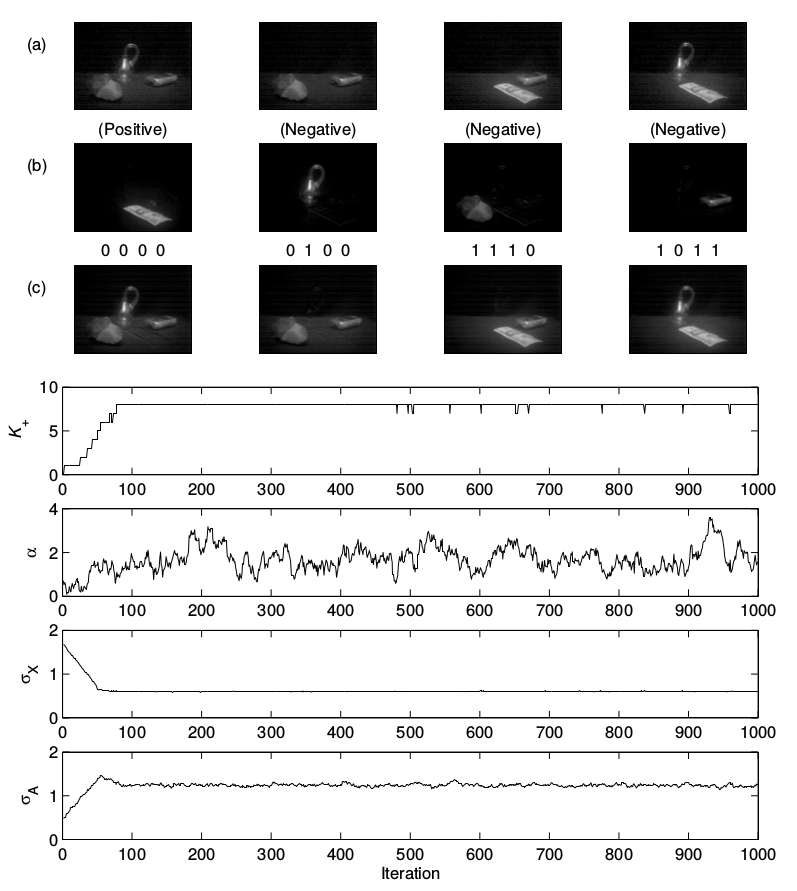
\includegraphics[scale=0.40]{exp}
    \caption{Caption me.\citet{Newman}}
  \label{fig:exp}
\end{figure}

The authors then apply this linear-Gaussian model to recover latent structure in image data. The dataset consists of one hundred $240 \times 320$ pixel images of four objects: a \$20 bill, a Klein bottle, a prehistoric handaxe, and a cellular phone. The objects are placed at a fixed location in each image, with some variation caused by hand placement. The data vector $\mathbf{x}_i$ for the $i$th image was a 100-dimensional vector consisting of the weights of the mean image and the first 99 principle components of the $i$th image. In this setup, each object is a latent feature $z_{ik}$ responsible for generating the observed pixel values in the image.

The results of posterior inference are shown in Figure \ref{fig:exp} for the first 1000 iterations of MCMC. Besides using the Gibbs sampler to infer the matrix $\mathbf{Z}$, the authors add Metropolis steps to estimate $\alpha$, $\sigma_x,$ and $\sigma_a$. The values of these hyperparameters/paramters are shown in Figure \ref{fig:exp} (bottom). Despite knowing that that there are four features responsible for generating the pixels, the model converges on seven features. This is not surprising; nonparametric models will tend to overestimate the number of parameters in a scenario where the true number of parameters is fixed.

Figure \ref{fig:exp} (a) shows example images from the dataset. Figure \ref{fig:exp} (b) shows the posterior mean of $\mathbf{a}_k$ for the four most frequent features in the 1000 iteration. These features appear to perfectly map to the presence/absence of the four objects when appropriately negated. The authors claim that the other three features discovered code for slight variations in location amount the objects.  Figure \ref{fig:exp} (c) shows the feature vector $\mathbf{z}_i$ for four test images along with the posterior means of the reconstructions of the images in (a) using the discovered features.

The authors also provide a comprehensive list of applications of the IBP to diverse applications in other works, including social science, genetics, networks, infinte Markov Models, and causality inference. The references for these examples are included in \citet{Griffiths2011}.

\bibliographystyle{apalike}
\bibliography{scribeadd, scribe}

\end{document}



